\section{Desenho Mecânico}

\begin{frame}{Frente}
    \begin{figure}
        \centering
        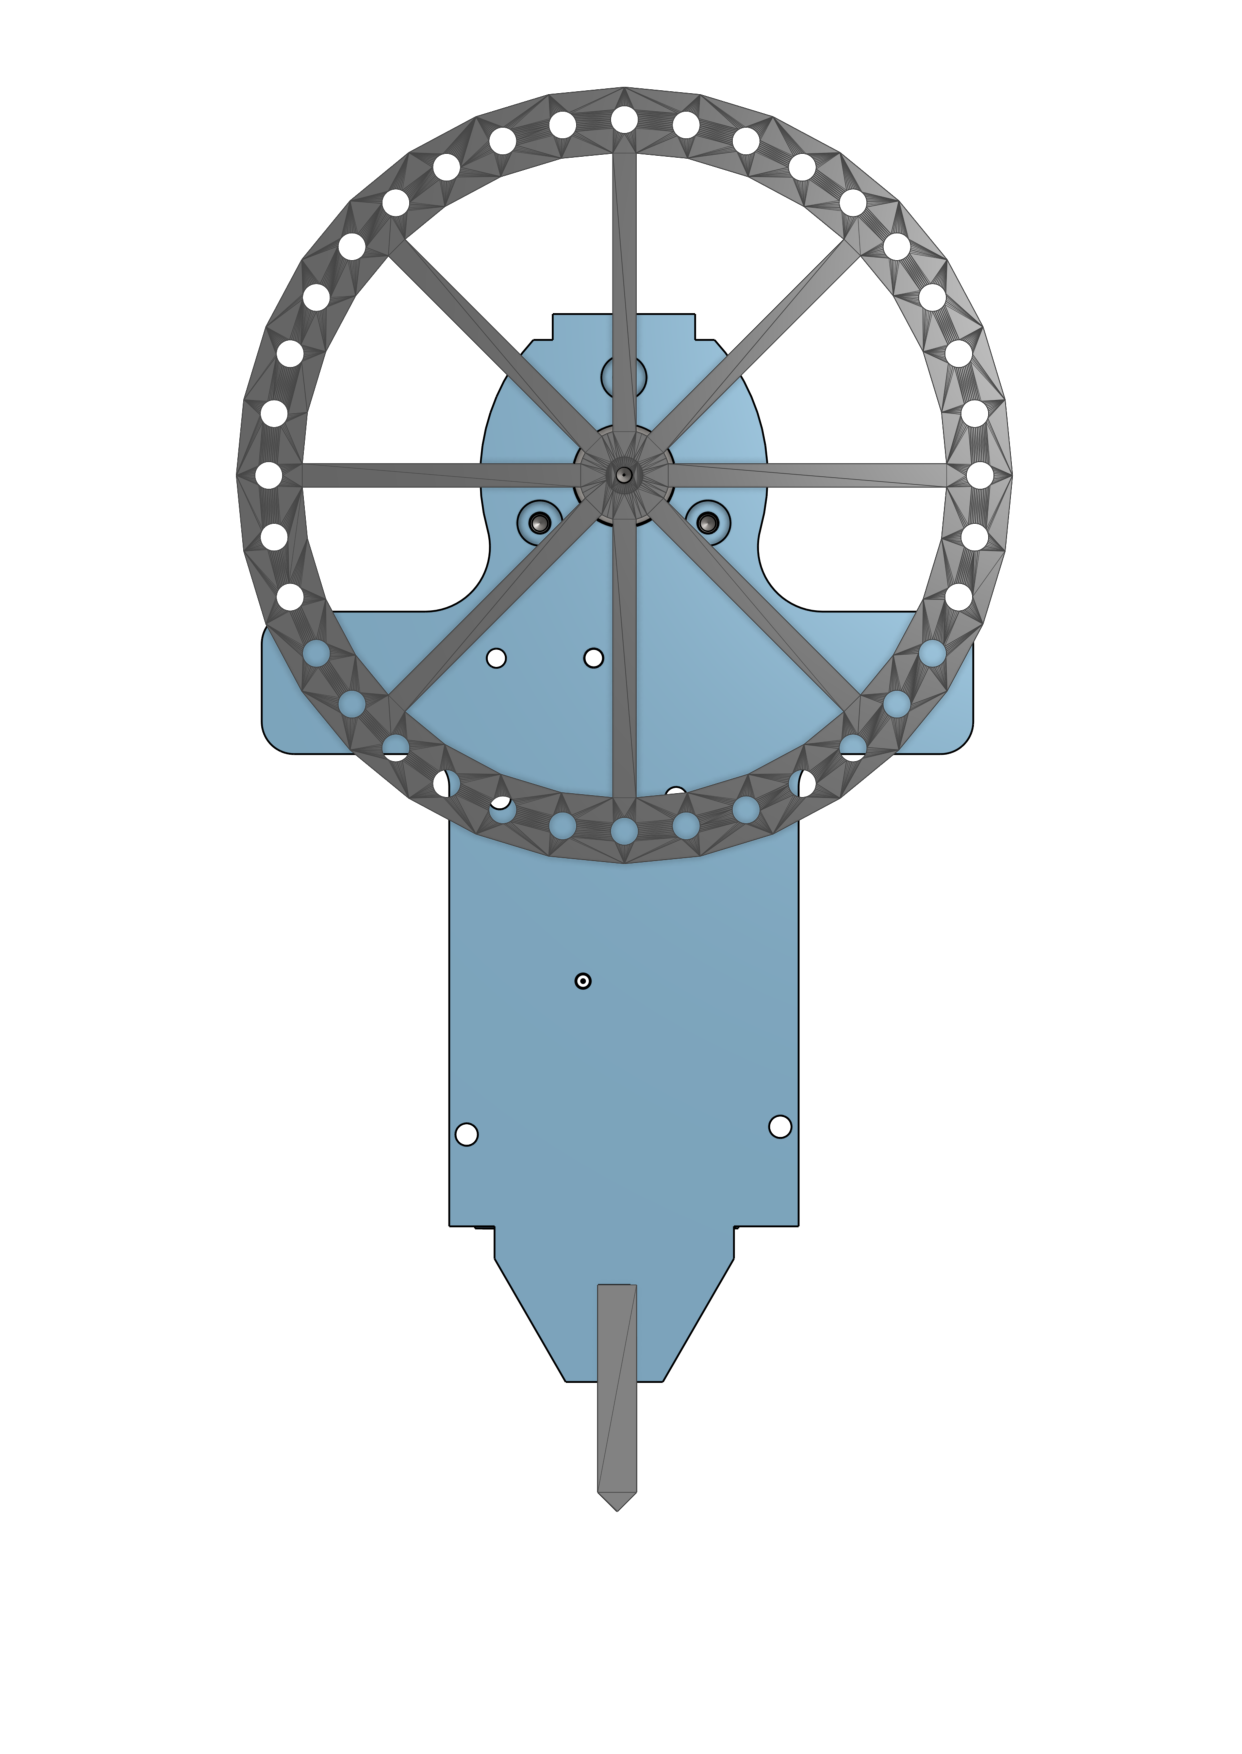
\includegraphics[height=0.8\textheight]{frente.pdf}
        \caption{Vista frontal do pêndulo invertido com roda de reação.}
        \label{fig:frente}
    \end{figure}
\end{frame}

\begin{frame}{Tras}
    \begin{figure}
        \centering
        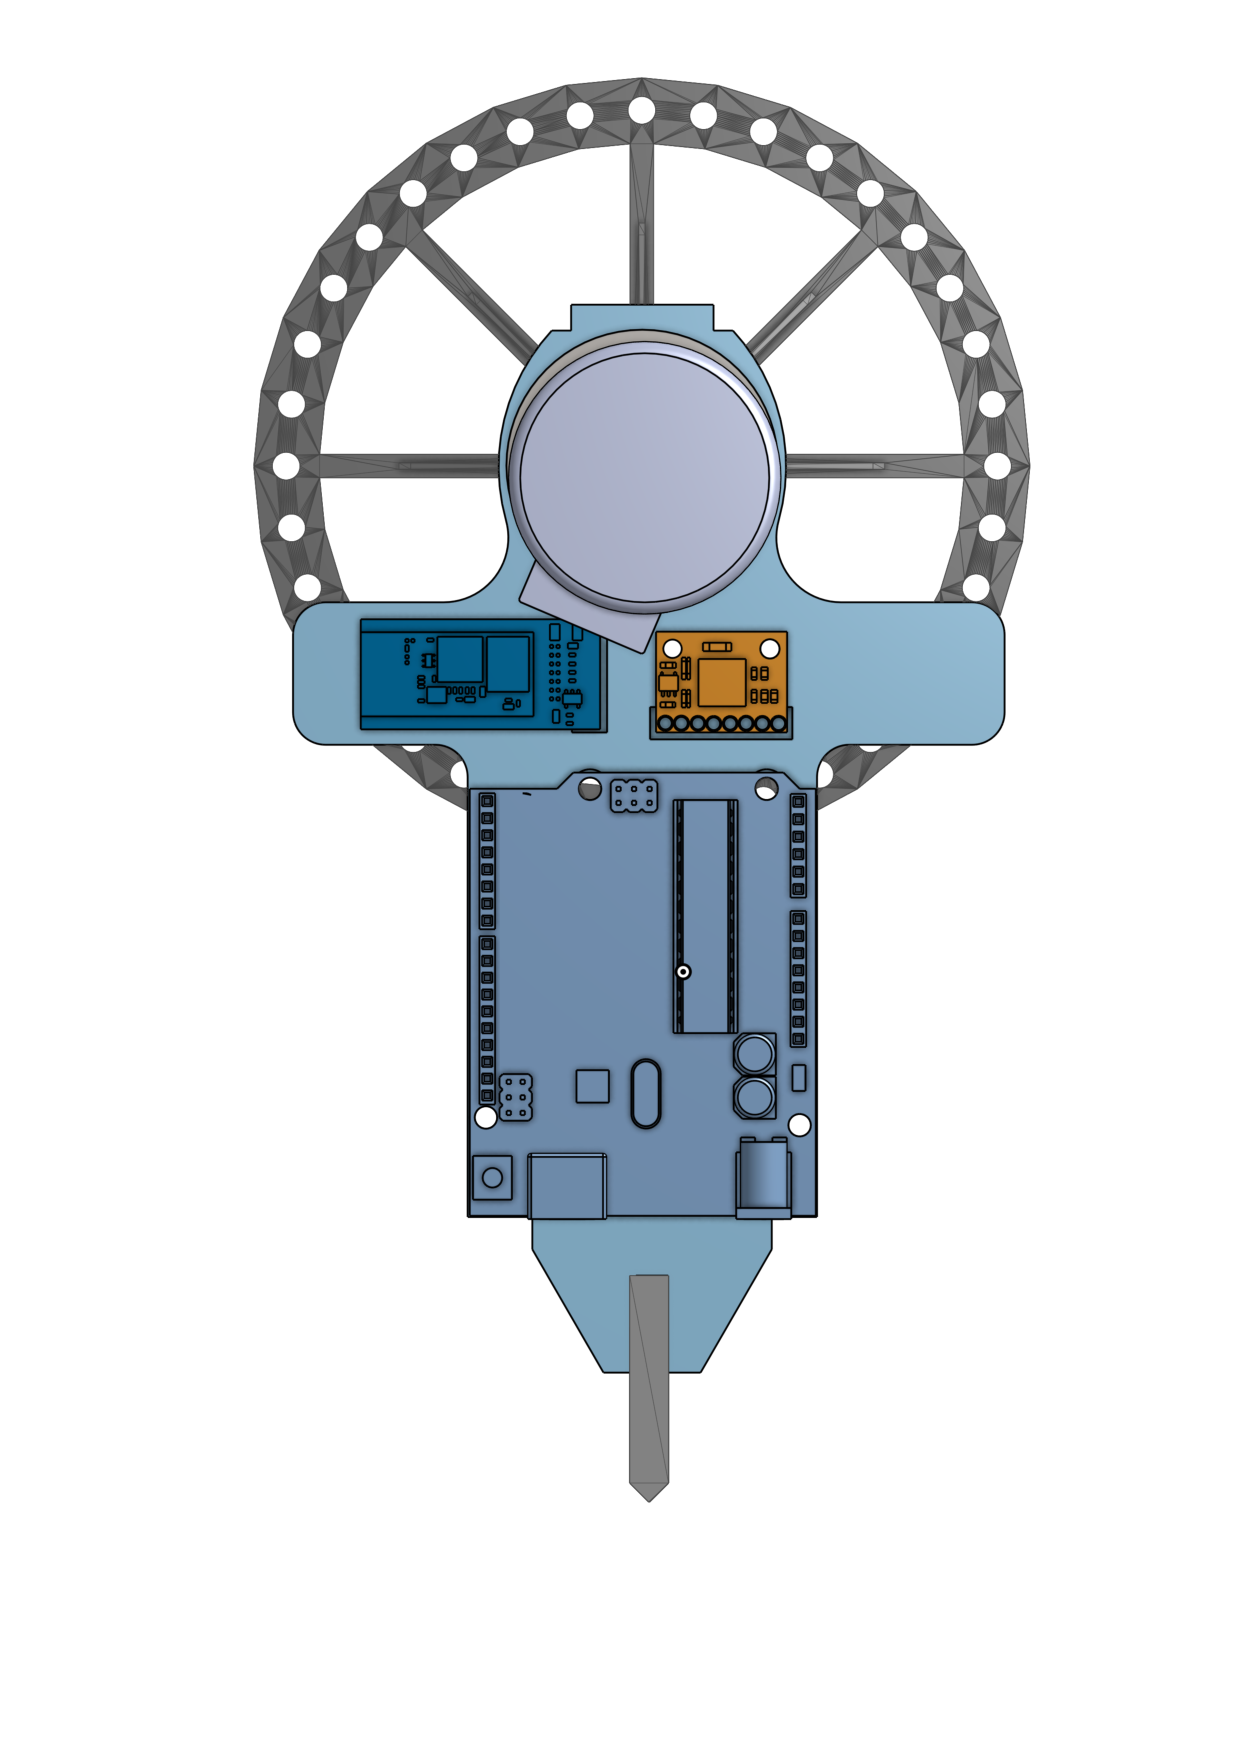
\includegraphics[height=0.8\textheight]{tras.pdf}
        \caption{Vista traseira do pêndulo invertido com roda de reação.}
        \label{fig:tras}
    \end{figure}
\end{frame}

\begin{frame}{Isométrica 1}
    \begin{figure}
        \centering
        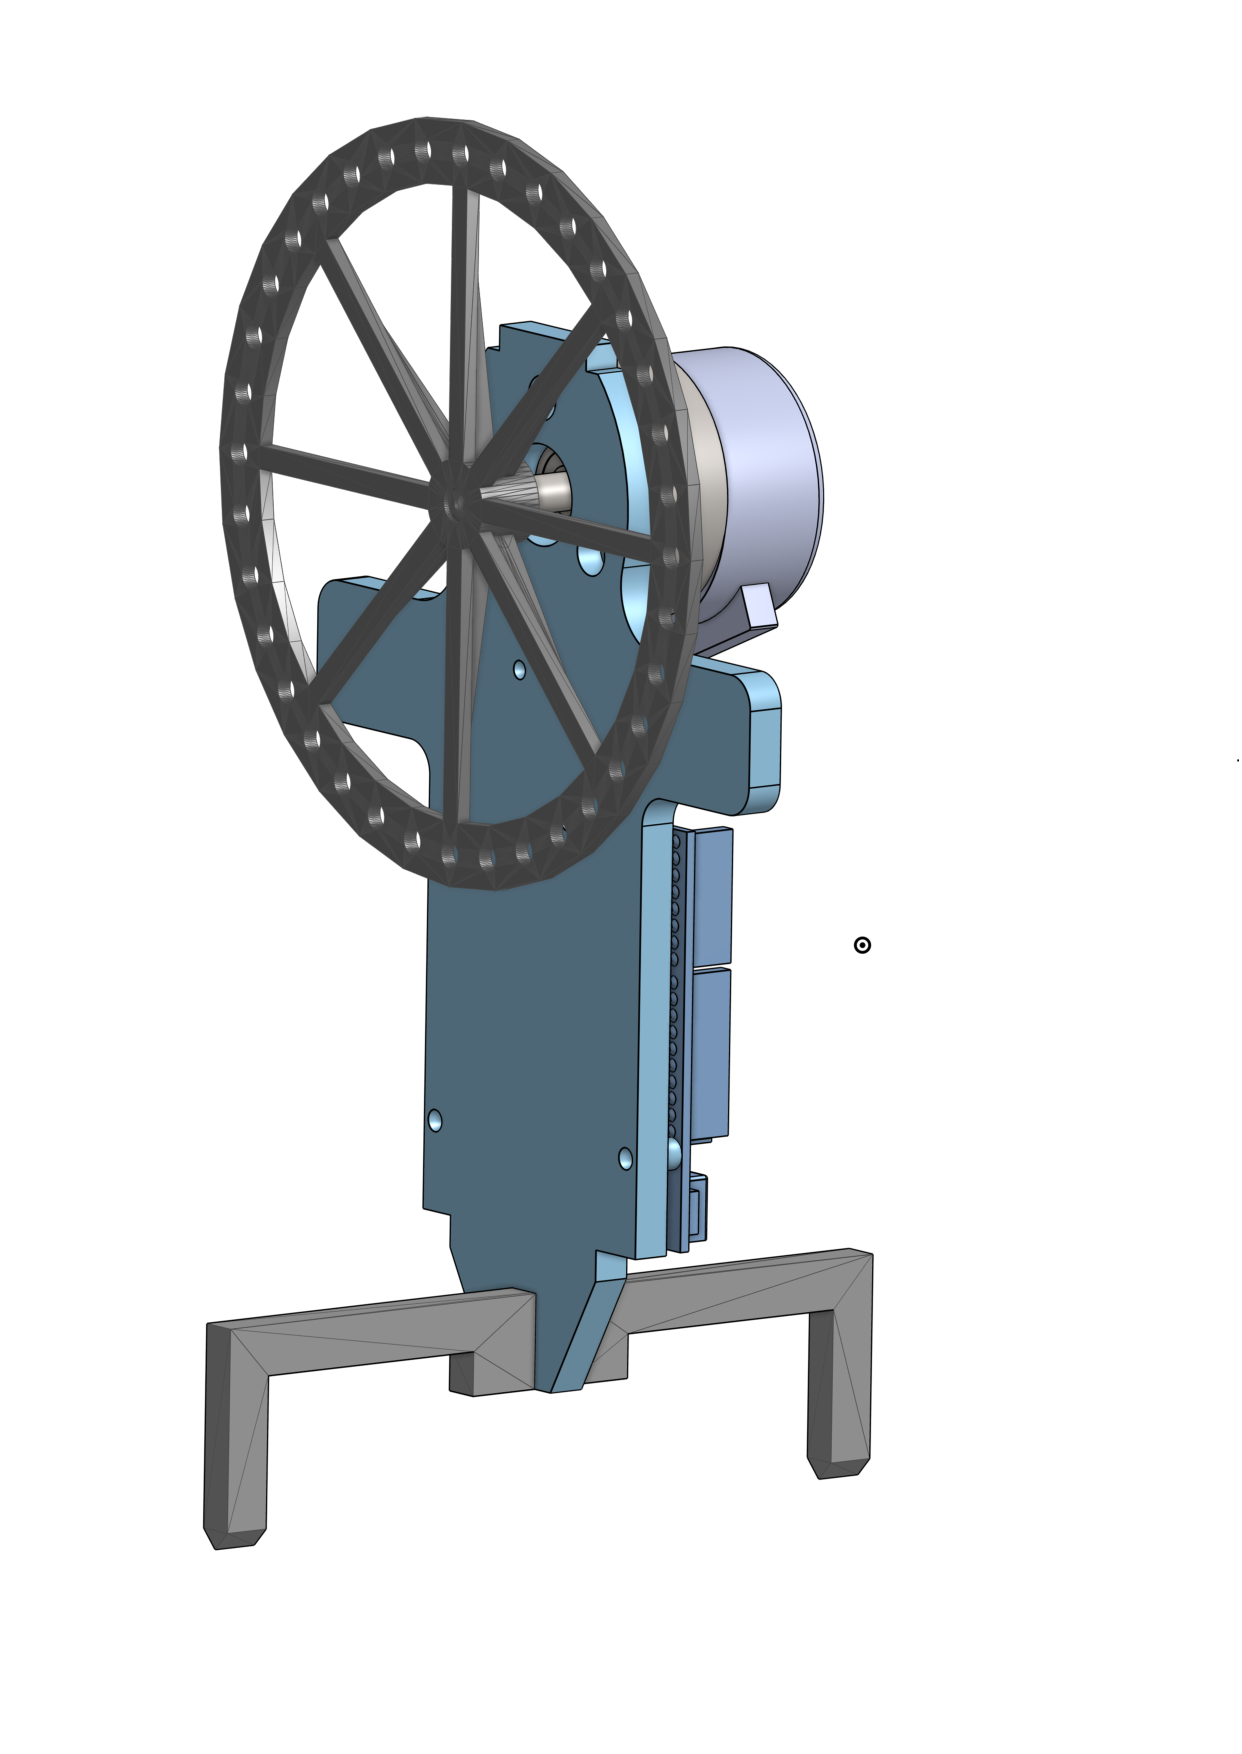
\includegraphics[height=0.8\textheight]{iso1.pdf}
        \caption{Vista isométrica do pêndulo invertido com roda de reação.}
        \label{fig:iso1}
    \end{figure}
\end{frame}

\begin{frame}{Isométrica 2}
    \begin{figure}
        \centering
        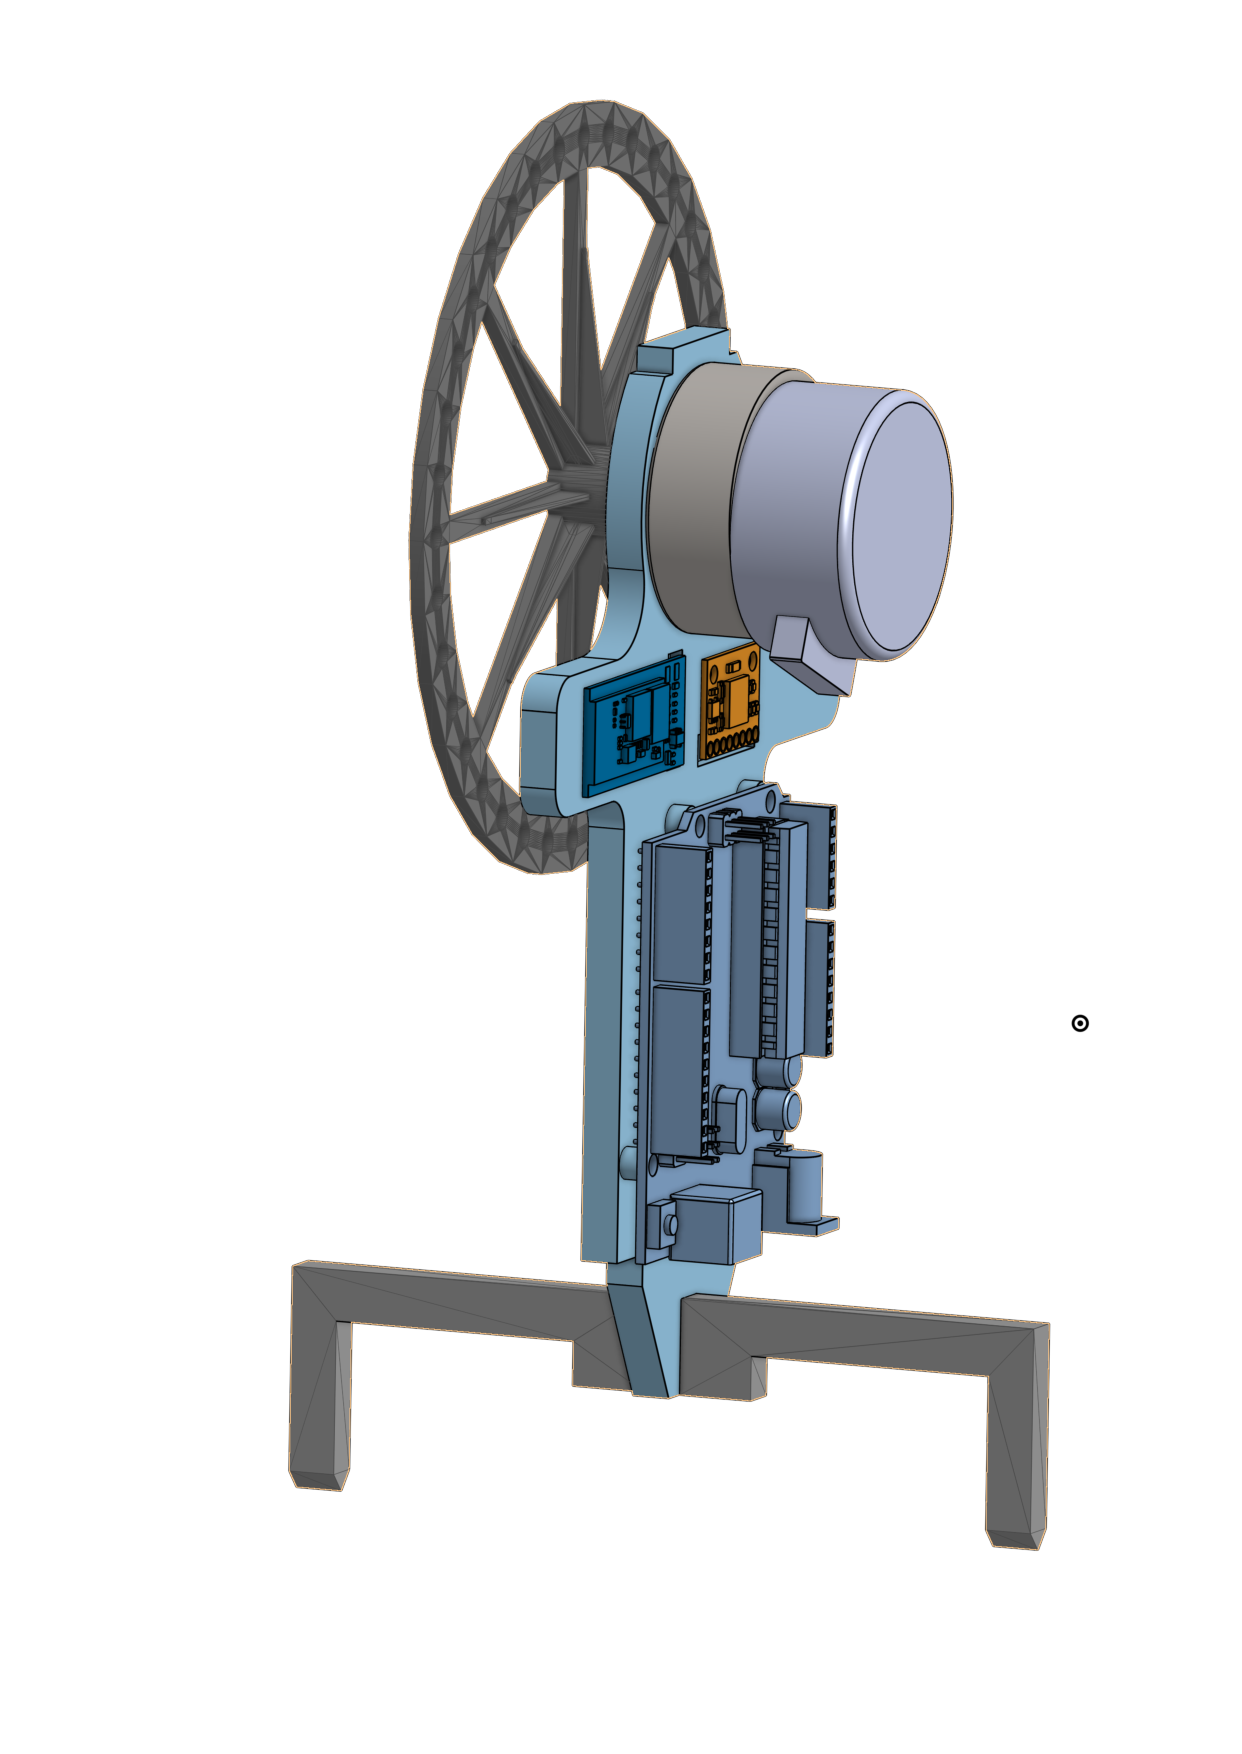
\includegraphics[height=0.8\textheight]{iso2.pdf}
        \caption{Outra vista isométrica do pêndulo invertido com roda de reação.}
        \label{fig:iso2}
    \end{figure}
\end{frame}
